%%%%%%%%%%%%%%%%%%%%%%%%%%%%%%%%%%%%%%%%%
% Article EcoFoG
% Version 2.1 (23/10/2017)
%
% adapté de :
% Stylish Article
% LaTeX Template
% Version 1.0 (31/1/13)
%
% This template has been downloaded from:
% http://www.LaTeXTemplates.com
%
% Original author:
% Mathias Legrand (legrand.mathias@gmail.com)
%
% License:
% CC BY-NC-SA 3.0 (http://creativecommons.org/licenses/by-nc-sa/3.0/)
%
%%%%%%%%%%%%%%%%%%%%%%%%%%%%%%%%%%%%%%%%%


%----------------------------------------------------------------------------------------
%	PACKAGES AND OTHER DOCUMENT CONFIGURATIONS
%----------------------------------------------------------------------------------------

\documentclass[fleqn,10pt]{ArtEcoFoG} % Document font size and equations flushed left

\setcounter{tocdepth}{3} % Show only three levels in the table of contents section: sections, subsections and subsubsections


% Pandoc environments
\usepackage{framed}
\usepackage{fancyvrb}
\providecommand{\tightlist}{%
  \setlength{\itemsep}{0pt}\setlength{\parskip}{0pt}}
\newcommand{\VerbBar}{|}
\newcommand{\VERB}{\Verb[commandchars=\\\{\}]}
\DefineVerbatimEnvironment{Highlighting}{Verbatim}{commandchars=\\\{\}, fontsize=\scriptsize} % Code R
\definecolor{shadecolor}{RGB}{248,248,248}
\newenvironment{Shaded}{\begin{snugshade}}{\end{snugshade}}
\newcommand{\KeywordTok}[1]{\textcolor[rgb]{0.13,0.29,0.53}{\textbf{{#1}}}}
\newcommand{\DataTypeTok}[1]{\textcolor[rgb]{0.13,0.29,0.53}{{#1}}}
\newcommand{\DecValTok}[1]{\textcolor[rgb]{0.00,0.00,0.81}{{#1}}}
\newcommand{\BaseNTok}[1]{\textcolor[rgb]{0.00,0.00,0.81}{{#1}}}
\newcommand{\FloatTok}[1]{\textcolor[rgb]{0.00,0.00,0.81}{{#1}}}
\newcommand{\ConstantTok}[1]{\textcolor[rgb]{0.00,0.00,0.00}{{#1}}}
\newcommand{\CharTok}[1]{\textcolor[rgb]{0.31,0.60,0.02}{{#1}}}
\newcommand{\SpecialCharTok}[1]{\textcolor[rgb]{0.00,0.00,0.00}{{#1}}}
\newcommand{\StringTok}[1]{\textcolor[rgb]{0.31,0.60,0.02}{{#1}}}
\newcommand{\VerbatimStringTok}[1]{\textcolor[rgb]{0.31,0.60,0.02}{{#1}}}
\newcommand{\SpecialStringTok}[1]{\textcolor[rgb]{0.31,0.60,0.02}{{#1}}}
\newcommand{\ImportTok}[1]{{#1}}
\newcommand{\CommentTok}[1]{\textcolor[rgb]{0.56,0.35,0.01}{\textit{{#1}}}}
\newcommand{\DocumentationTok}[1]{\textcolor[rgb]{0.56,0.35,0.01}{\textbf{\textit{{#1}}}}}
\newcommand{\AnnotationTok}[1]{\textcolor[rgb]{0.56,0.35,0.01}{\textbf{\textit{{#1}}}}}
\newcommand{\CommentVarTok}[1]{\textcolor[rgb]{0.56,0.35,0.01}{\textbf{\textit{{#1}}}}}
\newcommand{\OtherTok}[1]{\textcolor[rgb]{0.56,0.35,0.01}{{#1}}}
\newcommand{\FunctionTok}[1]{\textcolor[rgb]{0.00,0.00,0.00}{{#1}}}
\newcommand{\VariableTok}[1]{\textcolor[rgb]{0.00,0.00,0.00}{{#1}}}
\newcommand{\ControlFlowTok}[1]{\textcolor[rgb]{0.13,0.29,0.53}{\textbf{{#1}}}}
\newcommand{\OperatorTok}[1]{\textcolor[rgb]{0.81,0.36,0.00}{\textbf{{#1}}}}
\newcommand{\BuiltInTok}[1]{{#1}}
\newcommand{\ExtensionTok}[1]{{#1}}
\newcommand{\PreprocessorTok}[1]{\textcolor[rgb]{0.56,0.35,0.01}{\textit{{#1}}}}
\newcommand{\AttributeTok}[1]{\textcolor[rgb]{0.77,0.63,0.00}{{#1}}}
\newcommand{\RegionMarkerTok}[1]{{#1}}
\newcommand{\InformationTok}[1]{\textcolor[rgb]{0.56,0.35,0.01}{\textbf{\textit{{#1}}}}}
\newcommand{\WarningTok}[1]{\textcolor[rgb]{0.56,0.35,0.01}{\textbf{\textit{{#1}}}}}
\newcommand{\AlertTok}[1]{\textcolor[rgb]{0.94,0.16,0.16}{{#1}}}
\newcommand{\ErrorTok}[1]{\textcolor[rgb]{0.64,0.00,0.00}{\textbf{{#1}}}}
\newcommand{\NormalTok}[1]{{#1}}
\usepackage{longtable,booktabs}
\usepackage{caption}
% These lines are needed to make table captions work with longtable:
\makeatletter
\def\fnum@table{\tablename~\thetable}
\makeatother
% longtable 2 columns
% https://tex.stackexchange.com/questions/161431/how-to-solve-longtable-is-not-in-1-column-mode-error
\makeatletter
\let\oldlt\longtable
\let\endoldlt\endlongtable
\def\longtable{\@ifnextchar[\longtable@i \longtable@ii}
\def\longtable@i[#1]{\begin{figure}[t]
\onecolumn
\begin{minipage}{0.5\textwidth}\scriptsize
\oldlt[#1]
}
\def\longtable@ii{\begin{figure}[t]
\onecolumn
\begin{minipage}{0.5\textwidth}\scriptsize
\oldlt
}
\def\endlongtable{\endoldlt
\end{minipage}
\twocolumn
\end{figure}}
\makeatother

\usepackage{graphicx,grffile}
\makeatletter
\def\maxwidth{\ifdim\Gin@nat@width>\linewidth\linewidth\else\Gin@nat@width\fi}
\def\maxheight{\ifdim\Gin@nat@height>\textheight0.8\textheight\else\Gin@nat@height\fi}
\makeatother
% Scale images if necessary, so that they will not overflow the page
% margins by default, and it is still possible to overwrite the defaults
% using explicit options in \includegraphics[width, height, ...]{}
\setkeys{Gin}{width=\maxwidth,height=\maxheight,keepaspectratio}

% User-adder preamble
\usepackage{textcomp} \DeclareUnicodeCharacter{B0}{\textdegree}
\usepackage{tabu} \usepackage{caption}
\captionsetup{justification = justified}
\renewenvironment{table}{\begin{table*}}{\end{table*}\ignorespacesafterend}
\hyphenation{bio-di-ver-si-ty sap-lings re-or-gan-i-za-tion}

%----------------------------------------------------------------------------------------
%	ARTICLE INFORMATION
%----------------------------------------------------------------------------------------

\JournalInfo{Hal xxx} % Journal information
\Archive{DOI xxxx} % Additional notes (e.g. copyright, DOI, review/research article)

\PaperTitle{Post-Disturbance Tree Community Trajectories in a Neotropical Forest} % Article title

\Authors{
Ariane MIRABEL\textsuperscript{1*}\\ Eric Marcon\textsuperscript{1}\\ Bruno Hérault\textsuperscript{2 3}
} % Authors
\affiliation{
\textsuperscript{1}UMR EcoFoG, AgroParistech, CNRS, Cirad, INRA, Université des Antilles,
Université de Guyane.\\ \hspace{1em} Campus Agronomique, 97310 Kourou, France.\\\textsuperscript{2}Cirad, Univ montpellier, UR Forests \& Societies.\\ \hspace{1em} Montpellier, France.\\\textsuperscript{3}INPHB, Institut National Polytechnique Félix Houphouet-Boigny\\ \hspace{1em} Yamoussoukro, Ivory Coast.
}
\affiliation{*\textbf{Corresponding author}: ariane.mirabel@ecofog.gf, http://www.ecofog.gf/spip.php?article47} % Corresponding author

\Keywords{Taxonomic and Functional Biodiversity, Neotropical Forests, Disturbance Trajectories, Intermediate Disturbance Hypothesis, Long-term Resilience} % Keywords - if you don't want any simply remove all the text between the curly brackets
\newcommand{\keywordname}{Keywords} % Defines the keywords heading name

%----------------------------------------------------------------------------------------
%	ABSTRACT
%----------------------------------------------------------------------------------------

\Abstract{
Understanding the ecological rules underlying the maintenance of
tropical forests biodiversity, structure, functioning and dynamics is
urgent to anticipate their fate in the global change context. The huge
diversity of tropical forests is often assumed to be regularly reshaped
by natural disturbance yielding a diversity peak at intermediate
intensity, but this intermediate disturbance hypothesis (IDH) remains
debated, and this controversy also questions the extent of communities
resilience regarding their functional and taxonomic facets. To
disentangle the ecological processes driving community response to
disturbance, we analysed the taxonomic and functional diversity
trajectories following a disturbance gradient. Specifically, we
examined, over 30 years, the functional and taxonomic community
trajectories with regards to diversity, composition and redundancy.
Functional trajectories were drawn based on 7 leaf, stem and
life-history traits. We highlighted the cyclic recovery of community
taxonomic and functional composition. The pre-disturbance taxonomic
differences were maintained over time while the functional composition
trajectories were quite similar. The IDH did predict communities
functional diversity response while taxonomic diversity remained poorly
sensitive to disturbance intensity. Although consistent, the recovery of
community composition, diversity and redundancy remained unachieved
after 30 years. This acknowledged the need of decades-long cycles with
no disturbance to ensure a complete recovery, and questioned tropical
forest community resilience after repeated disturbance.
}

%----------------------------------------------------------------------------------------

\begin{document}

\selectlanguage{english}

\flushbottom % Makes all text pages the same height

\maketitle % Print the title and abstract box

\tableofcontents % Print the contents section

\thispagestyle{empty} % Removes page numbering from the first page

%----------------------------------------------------------------------------------------
%	ARTICLE CONTENTS
%----------------------------------------------------------------------------------------
























\section{Introduction}\label{introduction}

The large areas covered with tropical forests worldwide hold crucial
environmental, economic and social values. They provide wood and
multiple non-timber forest products, shelter a diversified fauna,
regulate the local and regional climates, the carbon, water and nutrient
cycles, and ensure cultural and human well-being. The growing demand in
forests products together with current global changes increases the
pressure on remaining natural forests
\citep{Gibson2011a, Morales-Hidalgo2015} and threatens the maintenance
and dynamics in space and time of communities structure, composition and
functioning \citep{Anderson-Teixeira2013, Sist2015}.

In tropical forests, ecological communities are regularly re-shaped by
natural disturbance events changing both the abiotic environment,
through the fluxes of light, heat and water \citep{Goulamoussene2017},
and the biotic interactions such as competition among species
\citep{Chesson2000, Herault2018}. One of the cornerstone of tropical
forest ecology is to understand the processes and drivers of ecosystems
response to disturbance \citep{White2001, Chazdon2003a}. For now, this
has been largely studied through forest structural parameters such as
aboveground biomass, tree height or stem density
\citep{Piponiot2016, Rutishauser2016} that are rapid and convenient to
measure. These structural parameters have been sucessfully modeled,
giving important insights into the recovery of ecosystem processes and
services \citep{Herault2018}. However the response of forests diversity
and composition is still unclear, albeit it determines the productivity,
stability and functioning of ecosystems \citep{Tilman2014, Liang2016}.
In the short-term, moderate disturbance may lead to positive impacts on
communities diversity, an idea formalized by the intermediate
disturbance hypothesis (IDH) stating a maximized species diversity when
disturbance intensity is not too high
\citep{Molino2001, Kariuki2006a, Berry2008a}.

Validations of the IDH though remain scarce in the long-term and mainly
rely on the analysis of taxonomic richness \citep{Molino2001}. Taxonomic
richness, alone, gives limited or misleading information on forests
recovery and functioning \citep{Martin2015, Chaudhary2016}. More
ecological-meaningful analysis would couple richness with (i) evenness
that would reveal underlying ecological processes and (ii) composition
that is crucial for conservation issues
\citep{Magurran1988, Lavorel2002, Bellwood2006}. Furthermore, a
functional approach accounting for species biological attributes would
directly link communities diversity, composition and redundancy to
ecosystem functioning and to its environmental constraints
\citep{Violle2007b, Moretti2009, Baraloto2012a, Scheiter2013}. In that
respect, the functional trait-based approach that focus on major traits
related to species ecology and mediate species performance in a given
environment was sucessfully adopted \citep{Diaz2005, Villeger2008a}. For
instance, the functional approach revealed in tropical rainforests the
deterministic processes entailing, after disturbance, a functional shift
from a dominance of ``conservative'' slow-growing species dealing with
scarce resources to ``acquisitive'' fast-growing species with rapid and
efficient use of abundant resources
\citep{TerSteege2001, Reich2014, Herault2011}. This shift is translated
into the trajectories of key functional traits related to resource
acquisition (leaf and stem traits) and life-history traits (seed mass,
maximum size)
\citep{Wright2004, TerSteege2006, Westoby2006a, Chave2009b}. Eventually
a complete overview of communities response to disturbance would
encompass the changes in functional redundancy, that quantifies the
amount of shared trait values among species \citep{Carmona2016}. The
high functional redundancy of hyperdiverse tropical forests
\citep{Bellwood2006} mitigates the impacts of species removal on
ecosystem functioning and determines the resilience of communities after
disturbance \citep{Trenbath1999, Elmqvist2003, Diaz2005}.

In this study, we monitored over 30 years the response of 75 ha of
neotropical forest plots set up on a gradient of disturbance intensity,
from 10 to 60\% of ecosystem above-ground biomass (AGB) removed. We made
use of a large functional traits database encompassing major leaf, stem
and life-history traits in order to draw the taxonomic and functional
trajectories in terms of richness, evenness, composition and redundancy
\citep{Lohbeck2015, Guariguata2001}. Specifically, we (i) questioned the
recovery of communities taxonomic and functional characteristics and
identified the underlying assembly processes, (ii) clarified the
validity of the IDH in the long term for tropical forest and elucidated
its translation into different trajectories, and (iii) questioned
community recovery time.

\section{Material and Methods}\label{material-and-methods}

\subsection{Study site}\label{study-site}

Paracou station in French Guiana (5\textdegree 18'N and
52\textdegree 53'W) is located in a lowland tropical rain forest in a
tropical wet climate with mean annual temperature of 26\textdegree C,
mean annual precipitation averaging 2980 mm.y\textsuperscript{-1} (30-y
period) and a 3-month dry season (\textless{} 100
mm.month\textsuperscript{-1}) from mid-August to mid-November, and a
one-month dry season in March \citep{Wagner2011}. Elevation ranges
between 5 and 50 m and soils correspond to thin acrisols over a layer of
transformed saprolite with low permeability generating lateral drainage
during heavy rains.

The experiment is a network of twelve 6.25ha plots that underwent a
disturbance gradient of three logging, thinning and fuelwood cutting
treatments (Table \ref{tab:Tab1}) according to a randomized plot design
with three replicate blocks of four plots. The disturbance corresponds
to averages of 10 trees removed per hectare with a diameter at 1.3 m
height (DBH) above 50 cm for treatment 1 (T1), 32 trees/ha above 40 cm
DBH for treatment 2 (T2) and 40 trees/ha above 40 cm DBH for treatment 3
(T3). Treatments T2 and T3 besides included the thinning of trees by
poison girdling \citep{Schmitt1990, Blanc2009}. The disturbance
intensity was measured as the percentage of aboveground biomass (\%AGB)
lost between the first inventory in 1984 and five years after
disturbance \citep{Piponiot2016} estimated with the BIOMASS R package
\citep{Biomass2018}.

\subsection{Inventories protocol and dataset
collection}\label{inventories-protocol-and-dataset-collection}

The study site corresponds to a tropical rainforest typical of the
Guiana Shield with a dominance of Fabaceae, Chrysobalanaceae,
Lecythidaceae and Sapotaceae. In the twelve experimental plots, all
trees above 10 cm DBH have been mapped and measured annually since 1984.
Trees are first identified with a vernacular name assigned by the forest
worker team, and afterward with a scientific name assigned by botanists
during regular botanical campaigns. In 1984, specific vernacular names
were given to 62 commercial or common species whereas more infrequent
ones were identified under general identifiers only distinguishing trees
and palm trees. From 2003, botanical campaigns have been conducted every
5 to 6 years to identify all trees at the species level but
identification levels still varied among plots and campaigns.

This variability of protocols in time raised methodological issues as
vernacular names usually correspond to different botanical species. It
resulted in significant taxonomic uncertainties that had to be
propagated to composition and diversity metrics. The uncertainty
propagation was done through a Bayesian framework reconstituting
complete inventories at genus level from real incomplete ones on the
basis of vernacular/botanical names association. Vernacular names were
replaced through multinomial trials based on the association probability
\(\big[\alpha_1, \alpha_2,..., \alpha_3\big]\) observed across all
inventories between each vernacular name \emph{v} and all species
\(\big[s_1, s_2,..., s_N\big]\):

\begin{align}
M_v\Big(\big[s_1, s_2,..., s_N\big],\big[\alpha_1, \alpha_2,..., \alpha_3\big]\Big) \nonumber
\end{align}

See appendix 1 and \citet{Aubry-Kientz2013} for the detailed
methodology.

Six functional traits representing leaf economics (leaves thickness,
toughness, total chlorophyll content and specific leaf area) and stem
economics (wood specific gravity and bark thickness), and life-history
traits (maximum specific height and seed mass) came from the BRIDGE
project \footnote{http://www.ecofog.gf/Bridge/}. Trait values were
assessed from a selection of individuals located in nine permanent plots
in French Guiana, including two in Paracou, and comprised 294 species
pertaining to 157 genera. Missing trait values (10\%) were filled using
multivariate imputation by chained equation \citep{Mice2011}.
Imputations were restricted within genus or family when samples were too
scarce, in order to account for the phylogenetic signal. Whenever a
species was not in the dataset, it was attributed a set of trait values
randomly sampled among species of the next higher taxonomic level (same
genus or family). As seed mass information was classified into classes,
no data filling process was applied and analyses were restricted to the
414 botanical species recorded.

All composition and diversity metrics were obtained after 50 iterations
of the uncertainty propagation framework.

\subsection{Composition and diversity
metrics}\label{composition-and-diversity-metrics}

To counter taxonomic uncertainties due to the variability of botanical
identification levels (in space) and protocols (in time), the taxonomic
composition and diversity analysis were conducted at the genus level.
Taxonomic and functional trajectories of community composition were
followed in a two-dimensional NMDS ordination space. Two NMDS using
abundance-based (Bray-Curtis) dissimilarity measures were conducted to
map either taxonomic or functional composition, the later based on the 7
leaf, stem and life history traits (without seed mass classes).
Trajectories along time were reported through the euclidean distance
between the target inventories and the reference inventories in 1989,
\emph{i.e.} 2 years after disturbance. Univariate trajectories of the
leaf, stem and life-history traits were also visualized with the
community weighted means (CWM) \citep{Diaz2007, Garnier2004}. Species
seed mass corresponded to 5 classes of increasing mass, seed mass
trajectories were therefore reported as the proportion of each class in
the inventories (Supp Mat XX).

The taxonomic diversity was reported through species richness and
evenness, \emph{i.e} the Hill number translation of the Simpson index
\citep{Hill1973}. These indices belong to the set of HCDT or generalized
entropy, respectively corresponding to the 0 and 2 order of diversity
(q), recomended for diversity studies
\citep{Patil1982, Tothmeresz1995, Marcon2015}. The functional diversity
was reported using the Rao index of quadratic entropy which combines
species abundance distribution and average pairwise dissimilarity based
on species functional traits.

The impacts of initial disturbance were tested with the spearman rank
correlation between the extrema of taxonomic and functional metrics
reached over the 30 years and the initial \%AGB removed. They were
besides analysed through polynomial regression between (i) taxonomic and
functional richness, evenness and diversity and (ii) the initial \%AGB
removed at 10, 20 and 30 years after disturbance.

The functional redundancy was measured as the overlap among species in
community functional space \citep{Carmona2016}. The samples of the trait
database were first mapped in a 2-dimensional plan with a PCA analysis.
Then, multivariate kernel density estimator associated with individual
trees returned species traits probability distribution (TDP). Species
TDP weighted by species abundance were eventually summed for each
community. Community functional redundancy was the sum of TDPs overlap,
expressed as the average number of species that could be removed from
without reducing the functional space (see appendix I for a more
comprehensive sheme).

\section{Results}\label{results}

\subsection{Communities richness and
evenness}\label{communities-richness-and-evenness}

From 1989 (2 years after disturbance) to 2015 (28 years after
disturbance), 828 388 individual trees and 591 botanical species
pertaining to 223 genus and 64 families were recorded. For undisturbed
plots, taxonomic Richness and Evenness remained stable over the 30 years
monitored. In disturbed communities, after low disturbance intensity the
taxonomic richness increased, reaching a maximum gain of 14 botanical
genera (plot 3 from treatment 2). After intense disturbance the
taxonomic richness followed a more complex trajectory, decreasing for
ten years after disturbance before recovering to pre-disturbance values.
The maximum richness loss or gain after disturbance was positively
correlated to the disturbance intensity
(\(\rho_{spearman}^{Richness}=0.50\)). In all disturbed plots the
taxonomic evenness first increased until a maximum reached after around
20 years. This maximum was positively correlated to the disturbance
intensity (\(\rho_{spearman}^{Evenness}=0.77\)). The evenness then
stabilized except for two T3 plots (plots 8 and 12) for which evenness
kept increasing.

\begin{figure*}

{\centering 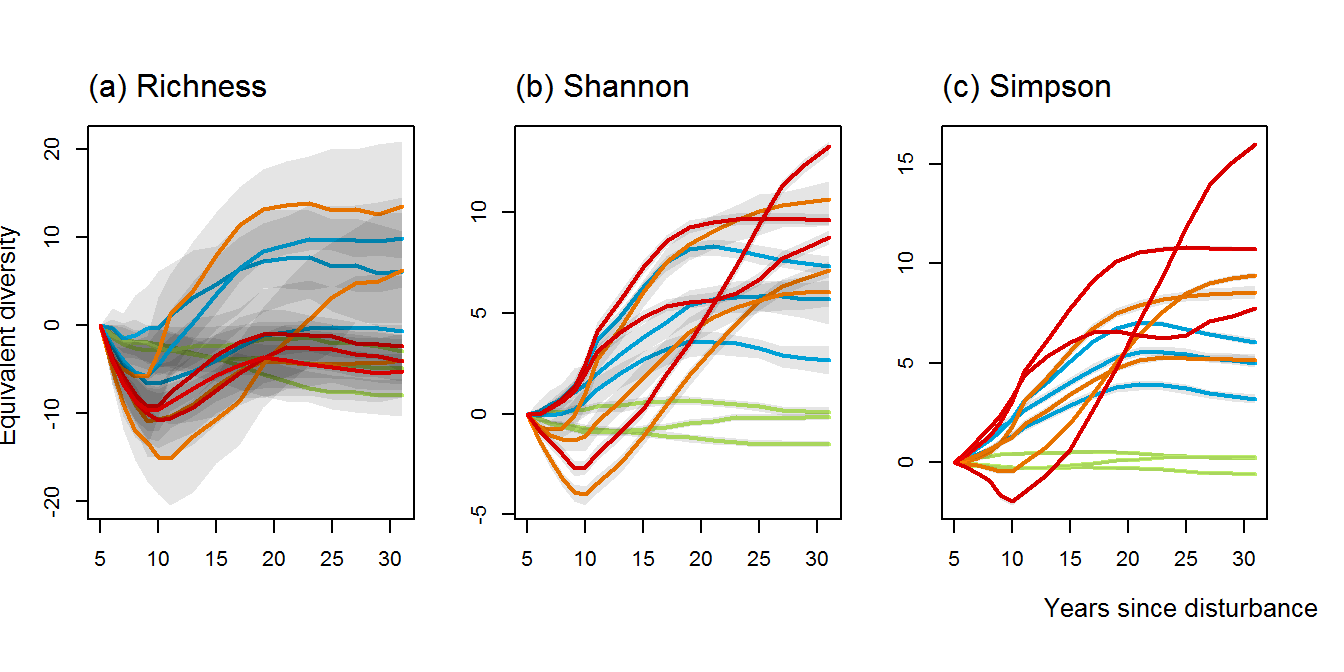
\includegraphics[width=1\linewidth]{WholePlotTrajectories_files/figure-latex/DivTaxo-1} 

}

\caption{Trajectories over 30 years of the difference with the 1989 inventory (2 years after disturbance) of community taxonomic \textbf{(a)} richness, \textbf{(b)}, taxonomic evenness and \textbf{(c)} functional diversity. Colors are treatments: green (control), blue (T1), orange (T2), red (T3) with shaded areas the credibility intervals }\label{fig:DivTaxo}
\end{figure*}

The plot 7 from treatment 1 displayed a constantly outlying functional
diversity and was removed from the graphical representation for better
readability (see appendix for full graphs). In undisturbed plots the
functional diversity remained stable along the 30 years. In disturbed
plots, trajectories depend on the disturbnace intensity with, for low
intensity, a low but long-lasting increase up to amximum reached after
20-25 years and, for, high intensity, a fast but short increase
followed, after 10 years, by a slow decrease towards the inital values.

Among polynomial regressions between (i) the \%AGB removed and (ii)
taxonomic richness, evenness and functional diversity after 10, 20 and
30 years the second degree better predicted the hump-shaped curve of the
disturbance impact in function of the intensity \ref{fig:IDHplot}. The
correlation with disturbance intensity was weak for the taxonomic
richness (\(R^2<0.37\)) and taxonomic evenness (\(R^2<0.43\)) but highly
significant for functional diversity (\(0.60<R^2<0.81\)).

\begin{figure*}

{\centering 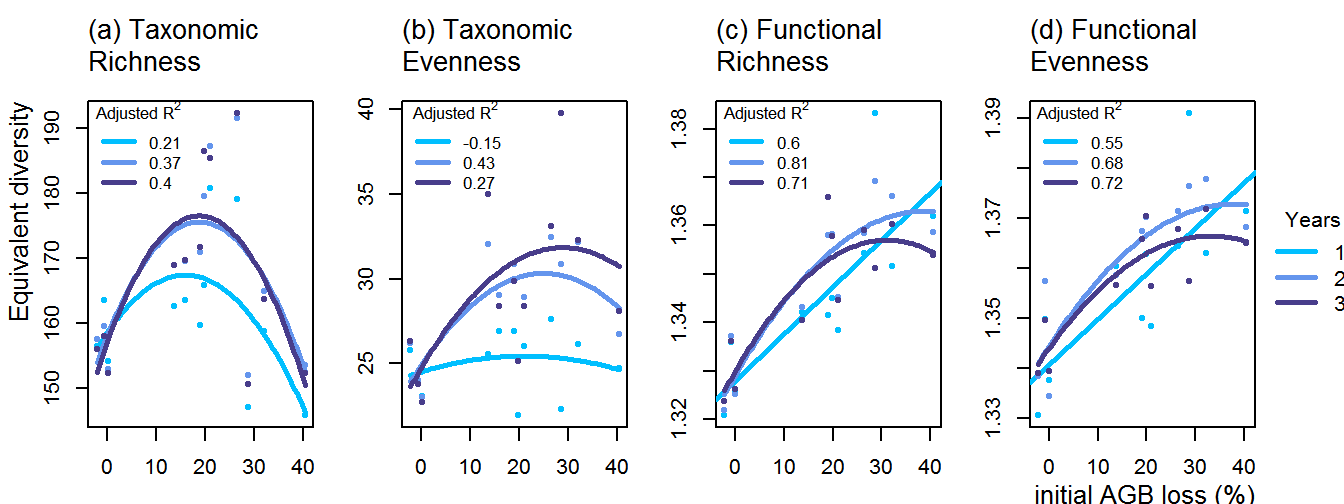
\includegraphics[width=1\linewidth]{WholePlotTrajectories_files/figure-latex/IDHplot-1} 

}

\caption{Relationship between the initial \%AGB removed and community taxonmic richness \textbf{(a)}, taxonomic evenness \textbf{(b)} and functional diversity \textbf{(c)} at 10, 20 and 30 years after disturbance. Colors are treatments: green (control), blue (T1), orange (T2), red (T3) with shaded areas the credibility intervals }\label{fig:IDHplot}
\end{figure*}

\subsection{Communities Composition}\label{communities-composition}

While both taxonomic and functional composition remained stable in
undisturbed communities (Figure \ref{fig:NMDSplans}), they followed
marked and consistent trajectories over post-disturbance time. in
disturbed communities, these compositional changes corresponded to
shifts towards species with more acquisitive functional strategies, from
communities with high average WSG to high average SLA and chlorophyll
content (see appendix I). For functional composition, this translated
into cyclic compositional changes with an unachieved recovery of the
initial composition (Figure \ref{fig:NMDSplans}). The maximum
dissimilarity with the initial state was positively correlated to the
disturbance intensity for both taxonomic and functional composition
(\(\rho_{spearman}^{taxonomic}=0.87\) and
\(\rho_{spearman}^{functional}=0.90\) respectively). The maximum value
was reached around 26 years after disturbance for taxonomic composition
and 22 years for functional composition.

\begin{figure*}

{\centering 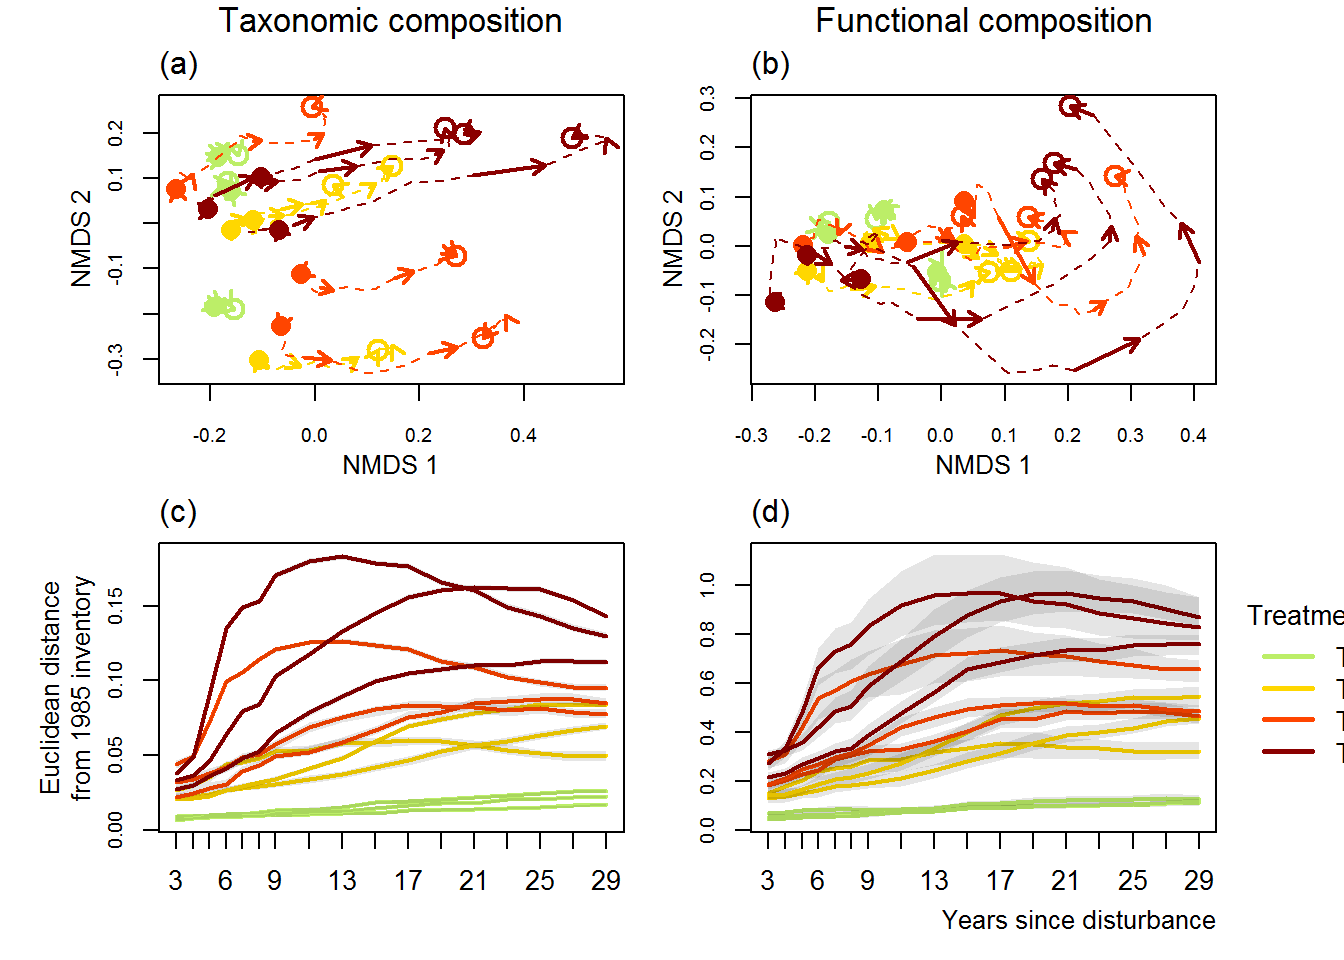
\includegraphics[width=1\linewidth]{WholePlotTrajectories_files/figure-latex/NMDSplans-1} 

}

\caption{Plot trajectories in terms of flora composition (left panels \textbf{(a)} and \textbf{(c)}) and functional composition (right panels \textbf{(b)} and \textbf{(d)}) in a two-dimensional NMDS space. Lower panels (\textbf{(c)} and \textbf{(d)}) represent the euclidean distance to initial condition along the 30 sampled years. Colors are treatments: green (control), blue (T1), orange (T2), red (T3) with shaded areas the credibility intervals}\label{fig:NMDSplans}
\end{figure*}

Except for leaf chlorophyll content, which continued to increase for
some T3 and T2 plots 30 years after disturbance, all traits and seed
mass proportions followed unimodal trajectories either stabilizing or
returning towards their initial values.

Maximum height at adult stage (\emph{Hmax}), leaf toughness
(\emph{L\_toughness}) and wood specific gravity (\emph{WSG}) first
decreased and then slightly increased but remained significantly lower
than their initial value (Figure \ref{fig:CWM}). On the other side, Bark
thickness (\emph{Bark\_thick}) and specific leaf area (\emph{SLA})
increased and while \emph{Bark\_thick} remained substantially high after
30 years, \emph{SLA} had almost recovered its initial value. For all
traits, the maximum difference to initial value was correlated to the
disturbance intensity (\(\rho_{spearman}^{L_{thickness}}=0.76\),
\(\rho_{spearman}^{L_{chloro}}=0.60\),
\(\rho_{spearman}^{L_{toughness}}=-0.53\),
\(\rho_{spearman}^{SLA}=0.93\), \(\rho_{spearman}^{WSG}=-0.75\),
\(\rho_{spearman}^{Bark-thickness}=0.71\),
\(\rho_{spearman}^{Hmax}=-0.40\)).

\begin{figure*}

{\centering 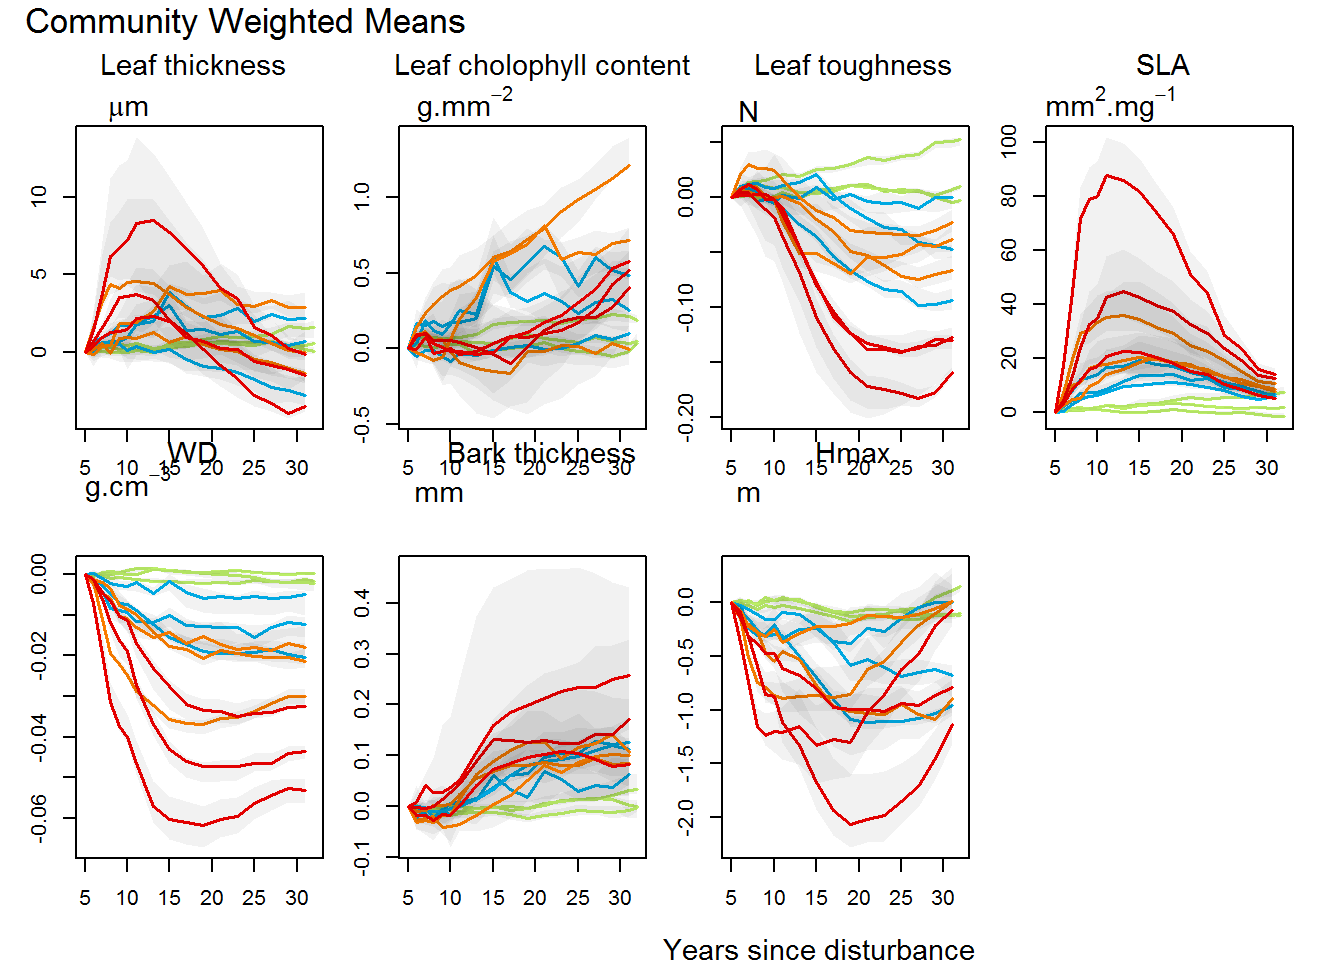
\includegraphics[width=1\linewidth]{WholePlotTrajectories_files/figure-latex/CWM-1} 

}

\caption{Trajectories of the communities weighted means (CWM) over 30 years after disturbance of 4 leaf traits (Leaf thickness, \emph{L\_thickness}, chlorophyll content, \emph{L\_chloro}, toughness, \emph{L\_toughness} and specific area, \emph{SLA}), 2 stem traits (wood specific gravity, \emph{WSG}, and bark thickness, \emph{Bark-thick}) and one life history trait (Specific maximum height at adult stage, \emph{Hmax}). Colors are treatments: green (control), blue (T1), orange (T2), red (T3) with shaded areas the credibility intervals.}\label{fig:CWM}
\end{figure*}

\subsection{Functional redundancy}\label{functional-redundancy}

All disturbed plots had lower functional redundancy than control plots
and followed similar hump-shaped trajectories (@ref(fig:RedFun\_rest)).
The maximum redundancy loss was positively correlated with the
disturbance intensity (\(\rho_{spearman}=0.47\)) and the initial value
had not recovered for any disturbed communities after 30 years.

\begin{figure}

{\centering 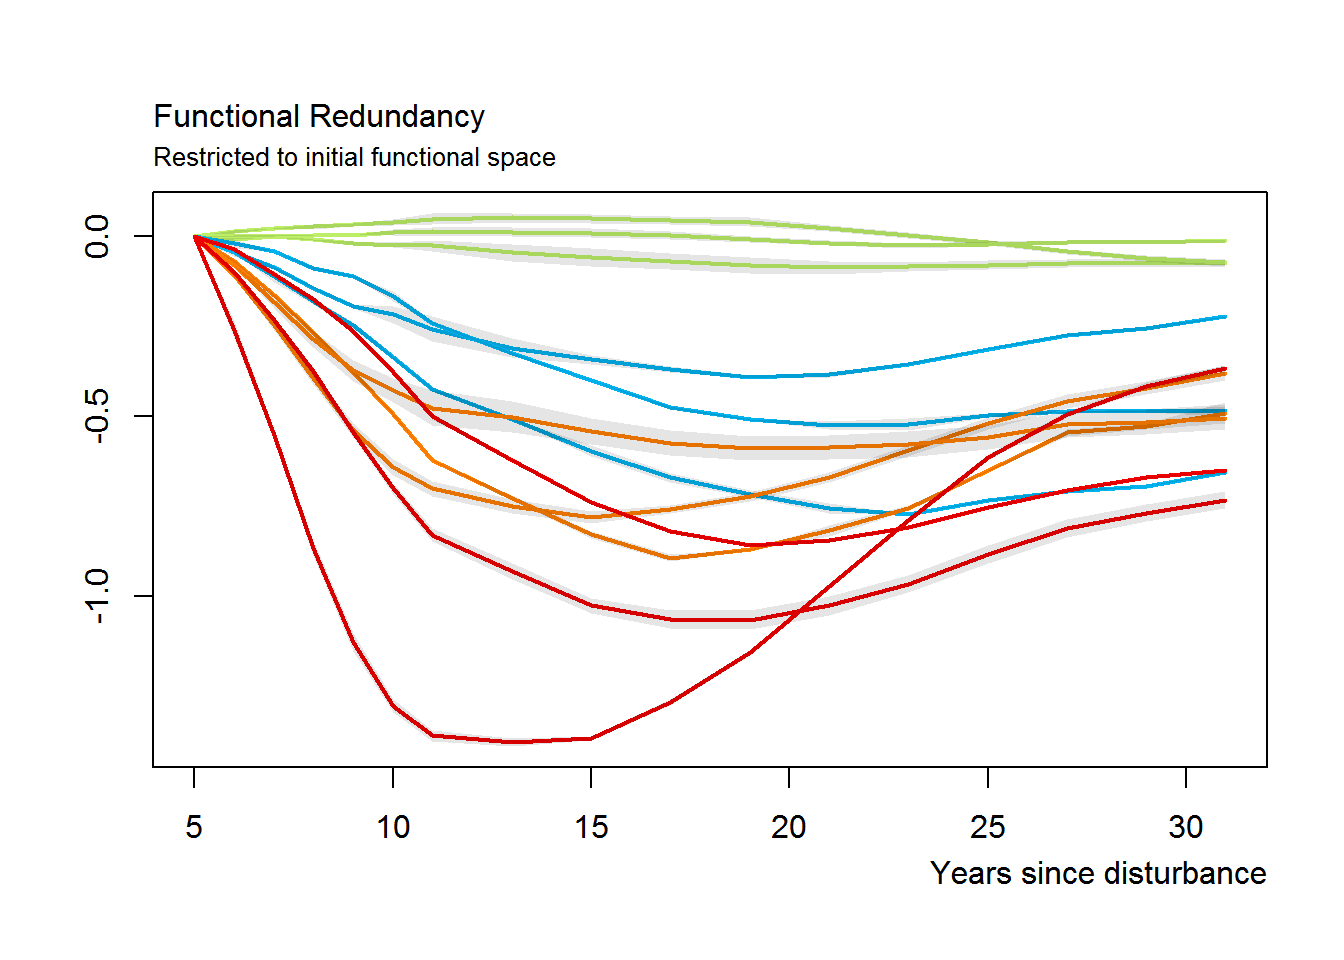
\includegraphics[width=1\linewidth]{WholePlotTrajectories_files/figure-latex/RedFun_rest-1} 

}

\caption{Trajectories of the functional redundancy within the initial functional space over 30 years after disturbance. Colors are disturbance treatments: green (control), blue (T1), orange (T2), red (T3) with shaded areas the credibility intervals.}(\#fig:RedFun_rest)
\end{figure}

\section{Discussion}\label{discussion}

\subsection{A cyclic recovery of community
composition}\label{a-cyclic-recovery-of-community-composition}

Communities taxonomic and functional composition appeared resilient,
following similar hump-shaped trajectories starting to return towards
pre-disturbance composition after 30 years. The taxonomic differences
among communities, marked before disturbance by the distinct starting
points on the NMDS axis 2, were maintained throughout recovery
trajectories. More than commonly thought, post-disturbance trajectories
depended on community initial composition, that partly determined the
pool of recruited species and constrained the trajectories towards the
initial composition. The high resilience of communities taxonomy
revealed that species not belonging to the pre-disturbance community
were hardly recruited because of the commonness of dispersal limitation
among tropical tree species (Svenning, Wright JECOL 2005).

Community functional composition followed similar trajectories that were
not so distinct in the functional space\ldots{}\ldots{}. Because the
pre-disturbance survivor trees mirror the initial communities
\citep{Herault2018}, the functional changes relied upon recruited trees
and the enhanced growth and survival of previously infrequent species
and functional types. Disturbance vacated environmental niches of high
light, space and nutrient availability, filled by competitive pioneers
that became dominant and determined the functional characteristics of
the community \citep{Grime1998}. Before disturbance and over communities
recovery time though, these species would be excluded by long-lived,
more resistant and shade tolerant species. The recovery of communities
functional characteristics, that mostly rely on dominant species
according to the ``vegetation quantity effect'' \citep{Grime1998},
suggested a similar recovery of the dominant species \citep{Molino2001}.
significant functional shifts towards resource-acquisitive strategies
(sharp increase in the SLA, leaf thickness and bark thickness and
decrease in wood specific gravity, leaf toughness and maximum height)
\citep{Westoby1998, Wright2004, Reich2014}.

\subsection{Another perspective on the intermediate disturbance
hypothesis}\label{another-perspective-on-the-intermediate-disturbance-hypothesis}

\begin{enumerate}
\def\labelenumi{\arabic{enumi}.}
\tightlist
\item
  IDH in Space (Disturbance gradient) The IDH consistently (predicted)
  the response of functional diversity to disturbance, but the theory
  was disproved regarding communities taxonomic richness and evenness.
  The functional range of species that could establish after disturbance
  was determined by the expanse of the environmental space made
  available by disturbance.
\end{enumerate}

In contrast the IDH translated in a decrease of the taxonomic richness
above an intensity threshold while the taxonomic evenness was decoupled
from disturbance intensity, as already observed in the Guiana Shield
\citep{Baraloto2012a} and in Bornean tropical forests
\citep{Cannon1998}. The taxonomic richness and evenness of recruited
species was fixed and at community scale the post-disturbance taxonomic
characterisitcs depended on the combination of these recruits and the
remaining pre-disturbance community.

The intensity of the disturbance determined the balance between trees
recruited in the pre-disturbance community and those recruited in
disturbance-specific community, functionally more diverse than
undisturbed forests but with lower taxonomic richness and higher
evenness.

\begin{enumerate}
\def\labelenumi{\arabic{enumi}.}
\setcounter{enumi}{1}
\tightlist
\item
  IDH in Time For the first years following disturbance community
  functional diversity increased through the filling of the vacated
  environmental space without competitive exclusion contraints. The
  maximum functional diversity was reached at the same time so the rate
  of space filling was similar among communities. The maximum was
  followed by the emergence of competitive exclusion processes bringing
  the functional diversity back to pre-disturbance levels and made the
  disturbance hypothesis intermediate in time.
\end{enumerate}

For medium disturbance intensity enhancing the taxonomic richness and
evennes, the taxonomic trajectories reached asymptots of high richness
and high evenness decoupled from their functional trajectories. Species
first established after disturbance remained in the community but became
less dominant, replaced the abundant pre-disturbance species, but the
recovery of rare species was hampered in the long-term
\citep{Hubbell2001, Chave2004}.

\subsection{The functional redundancy, key of the taxonomic
resilience}\label{the-functional-redundancy-key-of-the-taxonomic-resilience}

The recovery of the most infrequent species followed the lottery
recruitment rules \citep{Busing2002} and was hampered by the increasing
competition among species, implying long term recovery
\citep{Trenbath1999, Elmqvist2003, Diaz2005}.

Following disturbance the space and resources made available
corresponded to a rapid decrease of the functional redundancy within the
initial functional space. The high light, space and nutrient niches were
rapidly filled by species, mainly the most dominant and frequent ones.
Thereafter competitive exclusion emerged following the filling of the
niches and limited the recruitment of infrequent species
\citep{Busing2002}. The recovery of communities taxonomic richness and
evenness relied upon the recovery of the initial functional redudancy.
Although underway 30 years after disturbance the recovery remained
unachieved and after 30 years the recovery it was underway but remained
unachieved. This alteration of the functional redundancy meant a lower
resilience of pre-disturbance communities and higher chances to see the
persistence of disturbance-specific communities, with less species and
more pioneers \citep{Haddad2008, Burslem2000, Martin2013}. Besides the
slowed recovery of rare species increased the risks to loose cornerstone
specie, with unexpected ecological consequences
\citep{Jones1994, Chazdon2003a, Diaz2005, Gardner2007}. Apart from the
functional characteristics considered here, infrequent species mighthave
unique functions i nthe ecosystem or be a key for some fauna.

\section{Conclusions}\label{conclusions}

Our study revealed communities cyclic recovery after disturbance
allowing the resilience of their functioning and taxonomic composition
with the maintenance of initial differences among communities.
Communities functional evenness was enhanced for 20 years after
disturbance through the enrichment of the communities with pioneers and
light-demanding species,in accordance with the IDH. The IDH, though,
poorly predicted the disturbance impact on communities taxonomic
richness and evenness that were blurried by the emergence of competitive
exclusion along time. The resilience of tropical forests proved
consistent although spread over several decades. Still, the disturbance
impact on communities redundancy cautioned against the risks of
infrequent species loss and the persistence of disturbance-specific
communities \citep{Gourlet-Fleury2005}. As the trajectories highlighted
the recruitment processes proved central for communities response to
disturbance and closer focus on demographical drivers of communities
response would clarify the fate of the future forests.

%----------------------------------------------------------------------------------------
%	REFERENCE LIST
%----------------------------------------------------------------------------------------

\bibliographystyle{mee}
\makeatletter
% The filename has .bib extension the must be eliminated
\filename@parse{references.bib}
% parse stores the file name in base. Extension starts at the first dot, so don't use dots in file names.
\bibliography{\filename@base}
\makeatother


%----------------------------------------------------------------------------------------

\end{document}
